\documentclass[twoside,pl,final]{labman}

\usepackage{graphicx}
\usepackage{float}
\usepackage{url}
\usepackage{listings}
%\usepackage[caption=false]{subfig}
\usepackage{placeins}
\usepackage{subfig}

\graphicspath{ {fig/} }

\subject{Projektowanie układów analogowych dla systemów VLSI}
\title{Wzmacniacz operacyjny}
\author{mgr inż. Jakub Kopański}

\begin{document}
\maketitle
\tableofcontents
\clearpage
\listoffigures
\clearpage

\chapter{Wstęp}
\label{intro}
Wzmacniacze operacyjne są jednymi z podstawowych bloków
wykorzystywanych do budowania bardziej złożonych układów.
Ponieważ są tak powszechnymi elementami większych systemów,
omówimy dokładnie ich działanie oraz
zagadnienia związane z ich projektowaniem.

Wzmacniacz operacyjny przeznaczony jest do
pracy w układzie sprzężenia zwrotnego.
Dzięki temu o parametrach układu decydują
wartości elementów z których wykonano sprzężenie zwrotne,
a nie bezwzględne parametry wzmacniacza operacyjnego.
Takie rozwiązanie jest bardzo korzystne w realizacji scalonej
ponieważ o parametrach układu można decydować
stosunkiem wartości elementów sprzężenia.

\begin{figure}[!htbp]
  \centering
  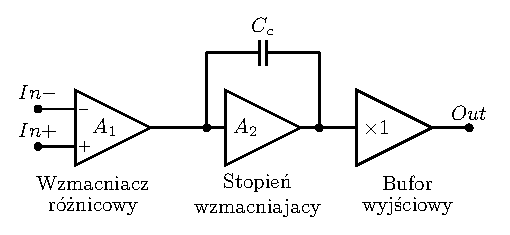
\includegraphics[width=0.9\textwidth]{idea}
  \caption{Schemat poglądowy wzmacniacza operacyjnego.}
  \label{fig:idea}
\end{figure}

Ideowy schemat wzmacniacza operacyjnego
zaprezentowano na~\fig{fig:idea}
Składa się on ze wzmacniacza różnicowego,
stopnia wzmacniającego oraz bufora wyjściowego.
Dzięki wzmacniaczowi różnicowemu mamy~2 wejścia wzmacniacza
(do jednego będziemy podawać sygnał sprzężenia zwrotnego).
Stopień wzmacniający zapewnia odpowiednio wysokie
wzmocnienie całego toru oraz dzięki kondensatorowi~$C_c$
kształtuje charakterystykę częstotliwościową wzmacniacza,
co będzie szerzej opisane w dalszej części instrukcji.
Ostatnim elementem jest bufor wyjściowy.
Zapewnia on małą rezystancje wyjściową wzmacniacza operacyjnego,
dzięki czemu możliwe jest obciążanie wzmacniacza \emph{małymi rezystancjami}.

W układach scalonych obciążenie rezystancyjne występuje bardzo rzadko.
Typowo wzmacniacze operacyjne muszą wysterować obciążenie
o charakterze pojemnościowym - bramkę tranzystora.
W takim przypadku można zrezygnować z bufora wyjściowego.
Tego typu wzmacniacz często nazywa się wzmacniaczem
transkonduktancyjnym~\emph{OTA} \eng{Operational Transconductance Amplifier}.
Rezygnując z bufora wyjściowego, należy zwrócić także uwagę na
ewentualne problemy ze \emph{slew rate} w szczególności gdy wartość
pojemności obciążająca wzmacniacz jest duża.
Ze względu na powszechność z jaką używa się wzmacniaczy~\emph{OTA}
w układach scalonych często nazywa się je wzmacniaczami operacyjnymi.

\chapter{Projektowanie wzmacniacza operacyjnego}
\label{opamp}

\section{Schemat elektryczny projektowanego układu}
\label{opamp:schematic}
\begin{figure}[!htbp]
  \centering
  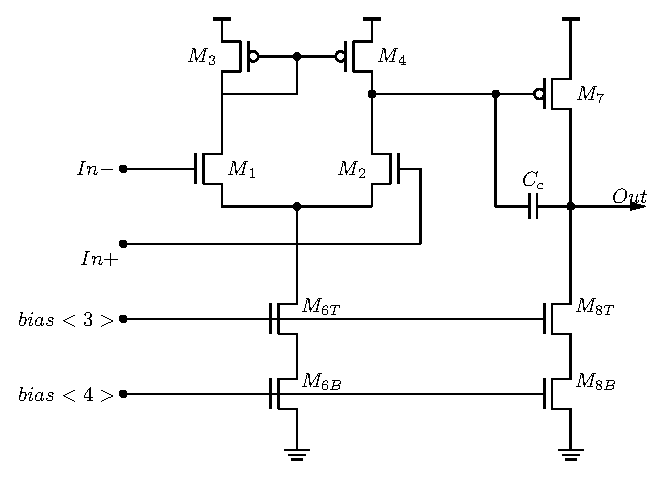
\includegraphics[width=0.9\textwidth]{schematic}
  \caption{Schemat elektryczny wzmacniacza operacyjnego.}
  \label{fig:schematic}
\end{figure}

Schemat układu jaki będziemy projektować
na zajęciach zaprezentowano na~\fig{fig:schematic}
Składa się ze wzmacniacza różnicowego który steruję
wzmacniaczem o wspólnym źródle.
Wzmocnienie układu w otwartej pętli, dla niskich częstotliwości
jest iloczynem wzmocnień poszczególnych stopni i wynosi:
\begin{equation}
  A_{OLDC} = A_1 \times A_2 =
    \overbrace{g_{mn} \cdot (r_{dsn} || r_{dsp})}^{A_1} \times
    \overbrace{g_{mp} \cdot r_{dsp}}^{A_2}
\end{equation}

\subsection{Punkt pracy}
\label{schematic:op}
Węzły \emph{bias<3>} i~\emph{bias<4>} pochodzą z bloku
projektowanego na poprzednich zajęciach.
Pary tranzystorów~$M_6$ i~$M_8$ tworzą źródła prądowe,
które wymuszają przepływ prądu w poszczególnych gałęziach układu.
Przez tranzystory $M_1$~i~$M_2$ płynie taki sam prąd,
równy połowie prądu lustra złożnonego z tranzystorów~$M_6$.
Bramki tranzystorów~$M_3$ i~$M_4$ są zwarte,
więc ich napięcia~$V_{GS}$ są takie same.
Ponieważ prąd płynący przez oba tranzystory jest taki sam,
napięcia~$V_{DS}$ obu tranzystorów muszą być takie same.
Dlatego napięcie~$V_{GS}$ tranzystora~$M7$,
tworzącego wzmacniacz drugiego stopnia,
jest równe napięciu~$V_{GS}$ tranzystorów~$M3$ i~$M4$.
Takie połączenie zapewni dobrze ustalony punkt pracy wzmacniacza.
Dzięki temu tranzystory będą posiadały znane parametry i możliwe
będzie przewidzenie osiągów projektowanego wzmacniacza operacyjnego.

\subsection{Wejściowe napięcie wspólne}
\label{schematic:cm}
Gdy wzmacniacz operacyjny pracuje przy
zamkniętej pętli sprzężenia zwrotnego,
napięcia na wejściach pary różnicowej są utrzymywane na tych samych
(lub prawie tych samych) wartościach.
Wartość średnia z napięć na obu wejściach wzmacniacza
nazywana jest napięciem wspólnym~\eng{common-mode voltage}.
Należy zastanowić się nad maksymalnym~$V_{CM_{max}}$ i
minimalnym~$V_{CM_{min}}$ napięciem wspólnym które zapewni,
że tranzystory wzmacniacza różnicowego pozostaną w nasyceniu.

Aby tranzystory źródła prądowego pozostały w nasyceniu
niezbędne jest napięcie co najmniej~$2V_{DSsat}$.
Stąd minimalne napięcie wspólne wynosi:
\begin{equation}
  V_{CM_{min}} = 2V_{DSsatn} + V_{GSn}
\end{equation}

Górny limit napięcia wspólnego można obliczyć zauważając,
że napięcie na drenie~$M_2$ i~$M_1$ jest równe i wynosi~$V_{DD} - V_{SGp}$.
Dlatego możemy zapisać:
\begin{equation}
  V_{DS} \geq V_{GS} - V_{THn} \rightarrow
  V_D \geq V_G - V_{THN} \rightarrow
  V_{CM_{max}} = V_{DD} - V_{SGp} + V_{THn}
\end{equation}

\subsection{Wejściowe napięcie różnicowe}
\label{schematic:diff}
Ponieważ prąd drenu tranzystora w zakresie nasycenia opisuję się równaniem:
\begin{equation}
  i_D = \frac{\beta_n}{2}(v_{GS} - V_{THN}),
\end{equation}
wejściowe napięcie różnicowe można przedstawić w postaci:
\begin{equation}
  v_{DI} = \sqrt{\frac{2}{\beta_n}}(\sqrt{i_{D1}} - \sqrt{i_{D2}}).
  \label{eqn:schematic:diff:di}
\end{equation}
Maksymalne wejściowe napięcie różnicowe otrzymamy podstawiając prąd źródła
prądowego~$I_{SS}$ płynącego w \emph{ogonie} pary różnicowej
za prąd~$i_{D1}$ do~(\ref{eqn:schematic:diff:di}) oraz zerując prąd~$i_{D2}$.
Otrzymamy wtedy:
\begin{equation}
  v_{DI_{max}} =
  v_{I1} - v_{I2} =
  \sqrt{\frac{2 \cdot L \cdot I_{SS}}{KP_n \cdot W}}
  \label{eqn:schematic:diff:di:max}
\end{equation}
Minimalne różnicowe napięcie wejściowe otrzymujemy poprzez
podstawienie prądu~$I_{SS}$ pod~$i_{D2}$ i wyzerowanie~$i_{D1}$.
\begin{equation}
  v_{DI_{min}} =
  - v_{DI_{max}} =
  - \sqrt{\frac{2 \cdot L \cdot I_{SS}}{KP_n \cdot W}}
\end{equation}

\section{Charakterystyka częstotliwościowa wzmacniacza}
\label{freq}
\begin{figure}[!htbp]
  \centering
  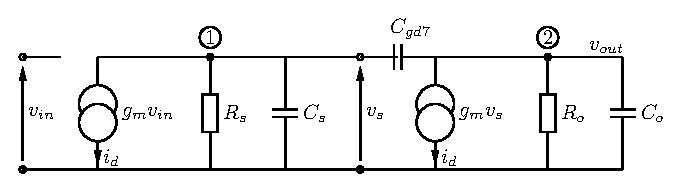
\includegraphics[width=0.9\textwidth]{smallsignal}
  \caption{Model małosygnałowy wzmacniacza operacyjnego.}
  \label{fig:smallsignal}
\end{figure}

Aby wyznaczyć charakterystykę częstotliwościową wzmacniacza posłużymy się
modelem małosygnałowym widocznym na~\fig{fig:smallsignal}
Wartości elementów schematu zastępczego wynoszą:
\begin{align}
  R_s &= r_{dsn} || r_{dsp}        \nonumber \\
  R_o &= r_{dsp} || R_{ocasn}      \nonumber \\
  g_{m1} &= g_{mn}                 \nonumber \\
  g_{m2} &= g_{mp}                 \nonumber \\
  C_s &= C_{ds4} + C_{gd2}         \nonumber \\
  C_o &= C_L + C_{gd8} \approx C_L \nonumber
\end{align}

Korzystając z twierdzenia Millera można przenieść
pojemność~$C_{gd7}$ na węzeł~$1$ i~$2$.
Wartości nowych pojemności wynoszą:
\begin{align}
  C_{MI} &= C_{gd7}(1 + |A_2|)), \\
  C_{MO} &= C_{gd7}(1 + \frac{1}{|A_2|}). \\
\end{align}
Taki zabieg spowoduję, że w układzie będą
2 stałe czasowe związane z węzłami~$1$ i~$2$.
Schemat elektryczny odpowiadającego modelu
małosygnałowego pokazany jest na~\fig{fig:miller}
Częstotliwości graniczne związane z tymi stałymi czasowymi będą wynosić:
\begin{align}
  f_1 &= \frac{1}{2 \pi (C_{gs} + C_{gd7}(1 + |A_2|)) \cdot r_{ds2} || r_{ds4}}
  \label{eqn:freq:pole:low} \\
  f_2 &= \frac{1}{2 \pi (C_{gd8} + C_L + (1 + \frac{1}{|A_2|})C_{gd7}) \cdot
  r_{ds7} || R_{ocascn}}
  \label{eqn:freq:pole:high}
\end{align}

\begin{figure}[!htbp]
  \centering
  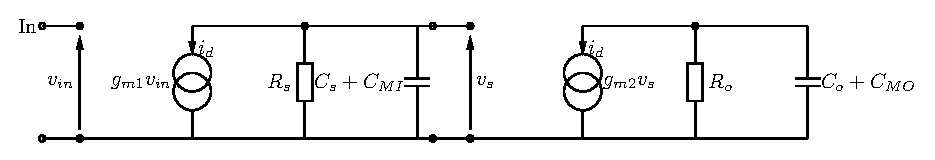
\includegraphics[width=0.9\textwidth]{miller}
  \caption{Model małosygnałowy po zastosowaniu efektu Millera.}
  \label{fig:miller}
\end{figure}

Charakterystyka częstotliwościowa układu z~\fig{fig:miller} ma postać:
\begin{equation}
  A_v(f) = \frac{\overbrace{g_{mn} \cdot (r_{dsn} || r_{dsp})}^{A_1} \times
                 \overbrace{g_{mp} \cdot r_{dsp}}^{A_2}}
                {\Big(1 + j \frac{f}{f_1}\Big)\Big(1 + j \frac{f}{f_2}\Big)}
\end{equation}

\subsection{Zero w prawej płaszczyźnie}
\label{freq:rhp}
Niestety model zaproponowany w rozdziale~\ref{freq}
nie jest całkowicie poprawny.
Stosując twierdzenie Millera, do wyznaczenia częstotliwości granicznych,
pomijane jest zero w charakterystyce częstotliwościowej.
Obserwując~\fig{fig:smallsignal} można zauważyć,
że w przypadku granicznym (dla bardzo wysokich częstotliwości)
pojemność~$C_{gd7}$ zwiera wejście z wyjściem drugiego stopnia wzmacniacza.
Dlatego w celu wyznaczenia dokładniejszej charakterystyki częstotliwościowej
nie możemy korzystać z twierdzenia Millera
oraz schematu zastępczego z~\fig{fig:miller}

W celu uproszczenia obliczeń potraktujemy węzeł~$1$
jako wejście rozważanego układu, do wyznaczenia częstotliwości zera.
Schemat zaprezentowano na~\fig{fig:smallsignal}
Suma prądów w węźle wyjściowym wynosi:
\begin{equation}
  \frac{v_{out} - v_s}{1 / j \omega C_{gd7}} +
  \frac{v_{out}}{R_o || 1 / j \omega C_o} +
  g_{m2} \cdot v_s = 0
\end{equation}
Wyznaczając wzmocnienie układu otrzymujemy równanie:
\begin{equation}
  \frac{v_{out}}{v_{s}} = -g_{m2} R_o \cdot
                          \frac{1 - j \omega \frac{C_{gd7}}{g_{m2}}}
                               {1 + j \omega ( C_{gd7} + C_o ) R_o},
  \label{eqn:freq:rhp:tf}
\end{equation}
skąd widzimy, że biegun jest taki sam jak w
równaniu~(\ref{eqn:freq:pole:high}).
Natomiast w liczniku transmitancji pojawiło się zero w prawej płaszczyźnie:
\begin{equation}
  f_z = \frac{g_{m2}}{2 \pi C_{gd7}}
  \label{eqn:freq:zero}
\end{equation}

Zero po prawej stronie układu współrzędnych
ma taki sam wpływ na odpowiedź amplitudową jak jak zero po lewej stronie,
ale inny wpływ na odpowiedź fazową.
Zero w prawej płaszczyźnie wpływa na odpowiedź fazową
tak samo jak biegun w lewej płaszczyźnie.
Ta właściwość rodzi ważne konsekwencje przy projektowaniu wzmacniaczy,
pracujących przy sprzężeniu zwrotnym (ale nie tylko!).
Wyjście wzmacniacza, przy dodatkowym przesunięciu fazy,
podane jako sprzężenie zwrotne może zmienić jego charakter
i zsumować się z sygnałem wejściowym
(dodanie sprzężenie zwrotne), powodując niestabilność wzmacniacza.

\subsection{Rozdzielanie biegunów}
\label{freq:split}

Użycie~(\ref{eqn:freq:pole:high}) do określenia położenia
wyjściowego bieguna jest obarczone błędem.
Wzmocnienie~$A_2$ maleje powyżej częstotliwości~$f_1$,
więc pojemność Millerowska~$C_{gd7}$ będzie mniejsza
niż w równaniu~\ref{eqn:freq:pole:high},
co spowoduję, że biegun wyjściowy będzie znajdował się
na znacznie wyższej częstotliwości niż~$f_2$.

W celu opisania tego efektu posłużymy się
schematem z~\fig{fig:smallsignal}
Wzmocnienie drugiego stopnia wzmacniacza jest opisane
przez~(\ref{eqn:freq:rhp:tf}).
Natomiast suma prądów wpływających do węzła~$2$ wynosi:
\begin{equation}
  \frac{v_s}{R_s} +
  \frac{v_s}{1 / j \omega C_s} +
  \frac{v_s - v_{out}}{1 / 1 j \omega C_{gd7}} -
  g_{m1} v_{in} = 0,
  \label{eqn:freq:split:kirchoff}
\end{equation}
co pozwala wyznaczyć:
\begin{equation}
  v_s = \frac{v_{out} \cdot j \omega C_{gd7} - g_{m1} v_{in}}
        {\frac{1}{R_s} + j \omega C_s + j \omega C_{gd7}}.
  \label{eqn:freq:split:vs}
\end{equation}
Podstawiając~(\ref{eqn:freq:split:vs}) do~(\ref{eqn:freq:split:vs})
możemy wyznaczyć wzmocnienie układu:
\begin{align}
  \frac{v_{out}}{v_{in}} = \nonumber \\
  \frac{g_{m1} g_{m2} R_o R_s (1 - s \frac{C_{gd7}}{g_{m2}})}
    {s^2 R_o R_s (C_{gd7} C_o + C_{gd7} C_s + C_o C_s) +
    s[R_o (C_{gd7} + C_o) + R_s (C_{gd7} + C_s) + g_{m2} R_o R_s C_{gd7}] + 1}.
  \label{eqn:freq:split:tf}
\end{align}
Zero transmitancji układu położone jest na
częstotliwości określonej przez~(\ref{eqn:freq:zero}).
Dla niskich częstotliwości mianownik
transmitancji~(\ref{eqn:freq:split:tf})
jest w przybliżeniu (ponieważ~$s^2$ jest małe) równy:
\begin{equation}
  1 + j \omega [(C_{gd7} + C_o) R_o +
                (C_{gd7} + C_s) R_s +
                C_{gd7} g_{m2} R_o R_s],
  \label{eqn:freq:split:denom:lowf}
\end{equation}
więc biegun na niskich częstotliwościach jest położony na częstotliwości:
\begin{equation}
  f_1 \approx \frac{1}{2 \pi [(C_{gd7} + C_o) R_o +
                              (C_s + C_{gd7} (1 + |A_v|)) R_s]},
  \label{eqn:freq:split:pole:low}
\end{equation}
gdzie:~$A_v = g_{m2} R_o$.
Jeżeli pojemność millerowska~$C_{gd7} (1 + |A_v|)$ jest
znacznie większa od pozostałych, to możemy przyjąć, że:
\begin{equation}
  f_1 \approx \frac{1}{2 \pi C_{gd7} (1 + |A_v|) R_s}
  \label{eqn:freq:split:pole:low:approx}
\end{equation}
Żeby wyznaczyć położenie drugiego bieguna musimy
wyciągnąć czynnik~(\ref{eqn:freq:split:denom:lowf})
z mianownika~(\ref{eqn:freq:split:tf}):
\begin{align}
  (1 + s[(C_{gd7} + C_o) R_o +
         (C_{gd7} + C_s) R_s +
          C_{gd7} g_{m2} R_o R_s]) \times \nonumber \\
  \Big(1 + \frac{s^2 R_o R_s (C_{gd7} C_o + C_{gd7} C_s + C_o C_s)}
                {1 + s[(C_{gd7} + C_o) R_o +
                       (C_{gd7} + C_s) R_s +
                        C_{gd7} g_{m2} R_o R_s]}\Big)
\end{align}
Jest to równanie w postaci:
\begin{equation}
  (1 + j \cdot \frac{f}{f_1})(1 + j \cdot \frac{f}{f_2})
\end{equation}
Dzieląc licznik i mianownik przez~$s R_o R_s$, otrzymujemy:
\begin{equation}
  1 + j \cdot \frac{s(C_{gd7} C_o + C_{gd7} C_s + C_o C_s)}
    {1 / s R_o R_s + [(C_{gd7} + C_o) / R_s +
                      (C_{gd7} + C_s) / R_o + C_{gd7} g_{m2}]}
\end{equation}
W praktycznych realizacjach wzmacniaczy możemy założyć:~$g_m >> \frac{1}{r_o}$
(jeżeli tak nie jest to \emph{wzmocnienie własne}
tranzystora~$g_m r_o$ jest zbyt małe
aby było możliwe zbudowanie na nim użytecznego wzmacniacza).
Dlatego możemy zapisać:
\begin{equation}
  f_2 \approx \frac{g_{m2} C_{gd7}}{2 \pi (C_{gd7} C_o + C_{gd7} C_s + C_o C_s)}
  \label{eqn:freq:split:denom:highf}
\end{equation}

Warto zauważyć, że jeżeli umieścimy dodatkową pojemność:~$C_c$
równolegle z pojemnością tranzystora~$C_{gd7}$ tak,
że efektywna pojemność wyniesie~$C_c + C_{gd7}$ to
zgodnie z~(\ref{eqn:freq:split:denom:lowf})
biegun na niższej częstotliwości~$f_1$
przesunie się na jeszcze mniejszą częstotliwość.
Natomiast biegun~$f_2$ znajdzie się na jeszcze wyższej częstotliwości.
Stąd nazwa rozdzielanie biegunów.

\begin{figure}[!htbp]
  \centering
  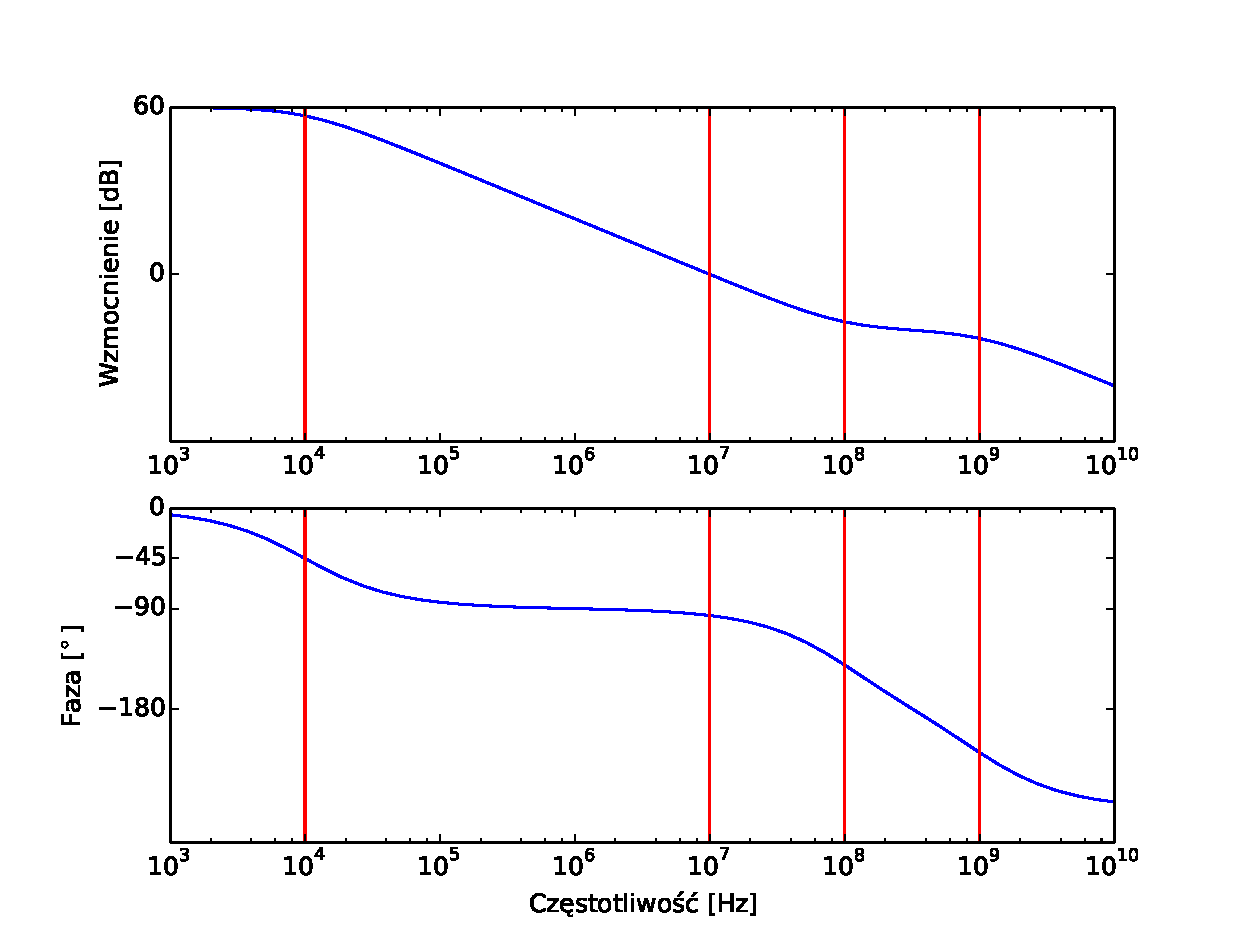
\includegraphics[width=0.9\textwidth]{tf}
  \caption{Typowe przebiegi wzmocnienia.}
  \label{fig:freq:split:tf}
\end{figure}

Częstą praktyką jest dodawanie pojemności~$C_c$ na tyle dużej aby biegun~$f_1$
był położony na znacznie niższej częstotliwości niż zero czy biegun~$f_2$.
Mówimy wtedy, że biegun związany z częstotliwością~$f_1$ jest
\emph{biegunem dominującym}.
W takim przypadku wzmocnienie możemy przybliżyć równaniem:
\begin{equation}
  A_v(f) = \frac{V_{out}(f)}{V_{in}(f)} \approx
  \frac{g_{m1} R_s g_{m2} R_o}{1 + j \frac{f}{f_1}} =
  \frac{g_{m1} R_s g_{m2} R_o}{1 + j 2 \pi f \cdot g_{m2} R_s R_o C_c}
  \label{eqn:freq:split:gain}
\end{equation}
Jest to równanie w postaci:
\begin{equation}
  A_V(f) = \frac{A_{DC}}{1 + j \frac{f}{f_{3dB}}},
\end{equation}
co pozwala nam zapisać:
\begin{align}
  A_{DC} &= g_{m1} R_s g_{m2} R_o
  \label{eqn:freq:split:dcgain} \\
  f_{3dB} &= \frac{1}{2 \pi g_{m2} R_s R_o C_c}
  \label{eqn:freq:split:bw}
\end{align}

Dla częstotliwości znacznie większych niż częstotliwość~$3$ decybelowa,
możemy przybliżyć transmitancje~\ref{eqn:freq:split:gain} poprzez:
\begin{equation}
  A_v \approx \frac{g_{m1}}{2 \pi f C_c},
\end{equation}
skąd możemy uzyskać zależność na częstotliwość
przy której wzmocnieni jest równe~$1$:
\begin{equation}
  f_{un} = \frac{g_m1}{2 \pi C_c}
  \label{eqn:freq:unity}
\end{equation}

\subsection{Usuwanie zera}
\label{freq:zero}

\begin{figure}[!htbp]
  \centering
  \subfloat[Usuwanie zera wzmacniaczem.]{
    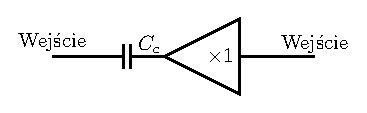
\includegraphics[width=0.4\textwidth]{zeros_amp}
    \label{fig:zero:amp}}
  \qquad
  \subfloat[Usuwanie zera rezystorem.]{
    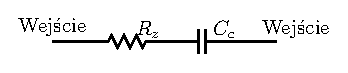
\includegraphics[width=0.4\textwidth]{zeros_res}
    \label{fig:zero:res}}
  \caption{Sposoby usuwania zera.}
  \label{fig:zero:cancel}
\end{figure}

Z~(\ref{eqn:freq:zero}) i~(\ref{eqn:freq:unity}) widać,
że jeżeli transkonduktancje obu tranzystorów są zbliżone to
częstotliwość zera oraz częstotliwość wzmocnienia jednostkowego
wypadają na takiej samej lub zbliżonej wartości.
Jak zostało wspomniane w rozdziale~\ref{freq:zero}
poprzez pojemność~$C_c$ może przechodzić sygnał z wejścia
bezpośrednio na wyjście wzmacniacza.
Jednocześnie zero w charakterystyce częstotliwościowej może spowodować,
że wzmocnienie będzie większe od~$1$ przy braku odwracania fazy sygnału.
Taka sytuacja może doprowadzić do niestabilności wzmacniacza.
Żeby uniknąć takiej sytuacji możemy dodać wtórnik w sprzężeniu zwrotnym,
jak na~\fig{fig:zero:amp}
Dzięki takiemu zabiegowi nadal otrzymamy efekt rozdzielania biegunów,
ale nie będzie \emph{drogi} z wejścia na wyjście wzmacniacza.
Innym rozwiązaniem jest dodanie rezystora szeregowo z pojemnością sprzężenia
zwrotnego $C_c$, aby stłumić sygnały wysokoczęstotliwościowe.
Dodanie rezystora przesuwa zero na wyższą częstotliwość,
zgodnie z zależnością:
\begin{equation}
  f_z = \frac{1}{2 \pi C_c \frac{1}{g_m}} \xrightarrow{z rezystorem}
  f_z = \frac{1}{2 \pi C_c (\frac{1}{g_m} - R_z)}
\end{equation}

\bibliographystyle{IEEEtran}
\bibliography{IEEEabrv,bibliography}

\end{document}
